\documentclass[headsepline=true, abstracton]{scrartcl}

\usepackage[utf8]{inputenc}
%\usepackage[T1]{fontenc}

\usepackage{amssymb}
\usepackage{amsmath}
\usepackage{amsthm}
\usepackage{bm}

\usepackage{natbib}

\usepackage[table,xcdraw]{xcolor}

\usepackage{graphicx}

\usepackage{geometry}
\usepackage{float}

\usepackage{setspace}

\usepackage{url}
 
 
 
  
\begin{document}



\renewcommand{\refname}{Bibliography}


\onehalfspacing
\setlength{\headsep}{15mm}


\thispagestyle{plain}

\title{\Large \textbf{Appendix:} \\ Generative Dynamics of Supreme Court Citations: \\ Analysis with a New Statistical Model}
%\author{}
 % Toggle % below to blind and unblind the manuscript
%  \author[1]{Christian Schmid \thanks{cxs5700@psu.edu}}
%   \author[2]{Ted Hsuan Yun Chen\thanks{thc126@psu.edu}}
% \author[2]{Bruce A. Desmarais\thanks{bdesmarais@psu.edu}}
% \author[1]{David R. Hunter \thanks{dhunter@stat.psu.edu}}
% \affil[2]{Department of Political Science, Pennsylvania State University}
 %\affil[1]{Department of Statistics, Pennsylvania State University}

\author{%
  Christian S. Schmid\footnote{Department of Statistics, The Pennsylvania State University, schmid@psu.edu}%
  \and Ted Hsuan Yun Chen \footnote{Department of Political Science, The Pennsylvania State University, thc126@psu.edu}%
   \and Bruce A. Desmarais \footnote{Department of Political Science, The Pennsylvania State University, bdesmarais@psu.edu}%
%  \and David R. Hunter \footnote{Department of Statistics, The Pennsylvania State University, dhunter@stata.psu.edu}%
  }


\maketitle

\section{c-ERGM Estimation}

The normalizing constant in Equation 1 is intractable. For example, in the simple case of adding three cases to a network in which six cases already exists---like that depicted in Figure \ref{fig:ctergm}---there are 16,777,216 unique configurations of $C_t$ that could be observed. The typical Supreme Court term involves adding hundreds of cases to a network that already includes thousands of previous cases. This means that straightforward methods of maximum likelihood estimation (MLE) are infeasible with the c-ERGM. 

The common alternative relies on Monte Carlo methods to approximate the normalizing constant by simulating a large set of networks \citep{hunter2006inference,hummel2012improving}. The resulting estimator, the Monte Carlo MLE (MCMLE), is approximately consistent, meaning that it converges to the MLE as the sample size, i.e., the number of simulated networks, increases. However, one drawback is that with the number of nodes in the Supreme Court citation network being in the order of $10,000$, obtaining the MCMLE is computationally expensive \citep{schmid2017exponential} and the success of the algorithm heavily relies on the starting parameter vector $\theta_0$, which is ideally chosen in the proximity of the unknown MLE \citep{hummel2012improving}. The prevailing choice for $\theta_0$ is the maximum pseudo-likelihood estimation (MPLE) \citep{strauss1990pseudolikelihood}, a fast estimation method that is defined as maximizing the log product of the conditional probability of each citation (and non-citation), conditional on the other elements of the observed citation network. The joint probability of all citations is replaced by the product over conditional probabilities, which, as we demonstrated above, assume a logit form. The MPLE is simple to obtain, but does not guarantee a starting value close to the MLE \citep{SchmidHunter2020}. 

We estimate the MCMLE for every term of the c-ERGM between 1950 and 2015. While the network for the 1950 term consists of $1962$ nodes, the size of the network monotonically increases to $10,020$ nodes for the 2015 term, making estimation more challenging as the network grows. The growth in the network also serves as our reason for estimating a separate model for each term. First, the network is large, with each term introducing the potential for hundreds-of-thousands of new citations. This means we have the statistical power necessary to estimate a separate set of parameter values for each term. Second, based on the findings of \citet{shalizi2013consistency}, we know that the set of parameter values that best fits a network should change as more nodes are added to the network. This means it would be inappropriate to assume a constant set of parameter values as more cases are added each term. 

The MCMLE of networks up until the 90s was obtainable in a reasonable time frame starting at the MPLE and sampling $10,000$ networks to approximate the normalizing constant. However, the estimation of most networks in the 90s with the MPLE as starting values was not feasible in an reasonable time frame anymore. Instead, we improved the choice of starting value $\theta_0$ by fixing it at the MCMLE of the previous term $t-1$ and successfully obtained the MCMLE of the network at term $t$. But even this approach started to fail for networks around the turn of the millennium. Neither the MPLE nor the MCMLE of previous terms as starting values led to successful estimation, and neither did the Stepping algorithm \citep{hummel2012improving}. 
The MCMLE for these large citation networks was obtained by setting the starting value according to an approach introduced by \citet{SchmidHunter2020}. This method is based on the fact that the MLE of exponential family distributions is solely a function of the vector of sufficient statistics $h(C_t, C_{<t})$, meaning that the MLE of two networks $A$ and $B$ is equal if $h(A)=h(B)$. However, the MPLE of networks with the same sufficient statistics is not necessarily the same. Instead of starting the MCMLE algorithm at the network's MPLE, \citet{SchmidHunter2020} propose searching for a network $C_t^*$ using simulated annealing \citep{Kirkpatrick83}, with $h(C_t, C_{<t}) = h(C_t^*, C_{<t})$ and a weak dependence structure among unfixed ties. The MPLE of such a network is similar to the MLE, making it an effective starting value for the MCMLE algorithm.


\section{Goodness-of-Fit}
We evaluate the goodness-of-fit of the model following \citet{hunter2008goodness} by examining the distribution of four hyper statistics, e.g., the out- and indegree distribution and the distribution for two different edgewise shared partners statistics. OTP stands for \textit{outgoing two-paths} and refers to the number of cases $r$ that are cited by case $i$ and that cite case $j$, while $j$ is also directly cited by $i$. The second ESP statistic is the OSP specification that has been introduced in section 4.1.2 in the paper. Figure \ref{GOF} visualizes the goodness-of-fit results for the citation network for the 1950 (top) and 2015 (bottom) term. The solid black line indicates the statistic's distribution in the Supreme Court citation network of that given term and the boxplots depict the statistic's distribution of $1000$ networks that have been simulated from the ERGM defined by the MCMLE. This means that in the ideal case the solid black line passes through ever single boxplot.


We see that our models do a good job capturing the out and indegree distribution of the citation network, since the black line falls almost exclusively within the ranges spanned by the boxplots. For the ESP distributions we can observe that the number of ties with $r=0$ shared partners is captured well for both the OTP as well as for the OSP statistic. However, the model overestimates the number of $r=1$ shared partners and then, especially in the 2015 term network, underestimates the number of ties with more than $r=1$ shared partners. 

 \begin{figure}[H]
 \begin{center}
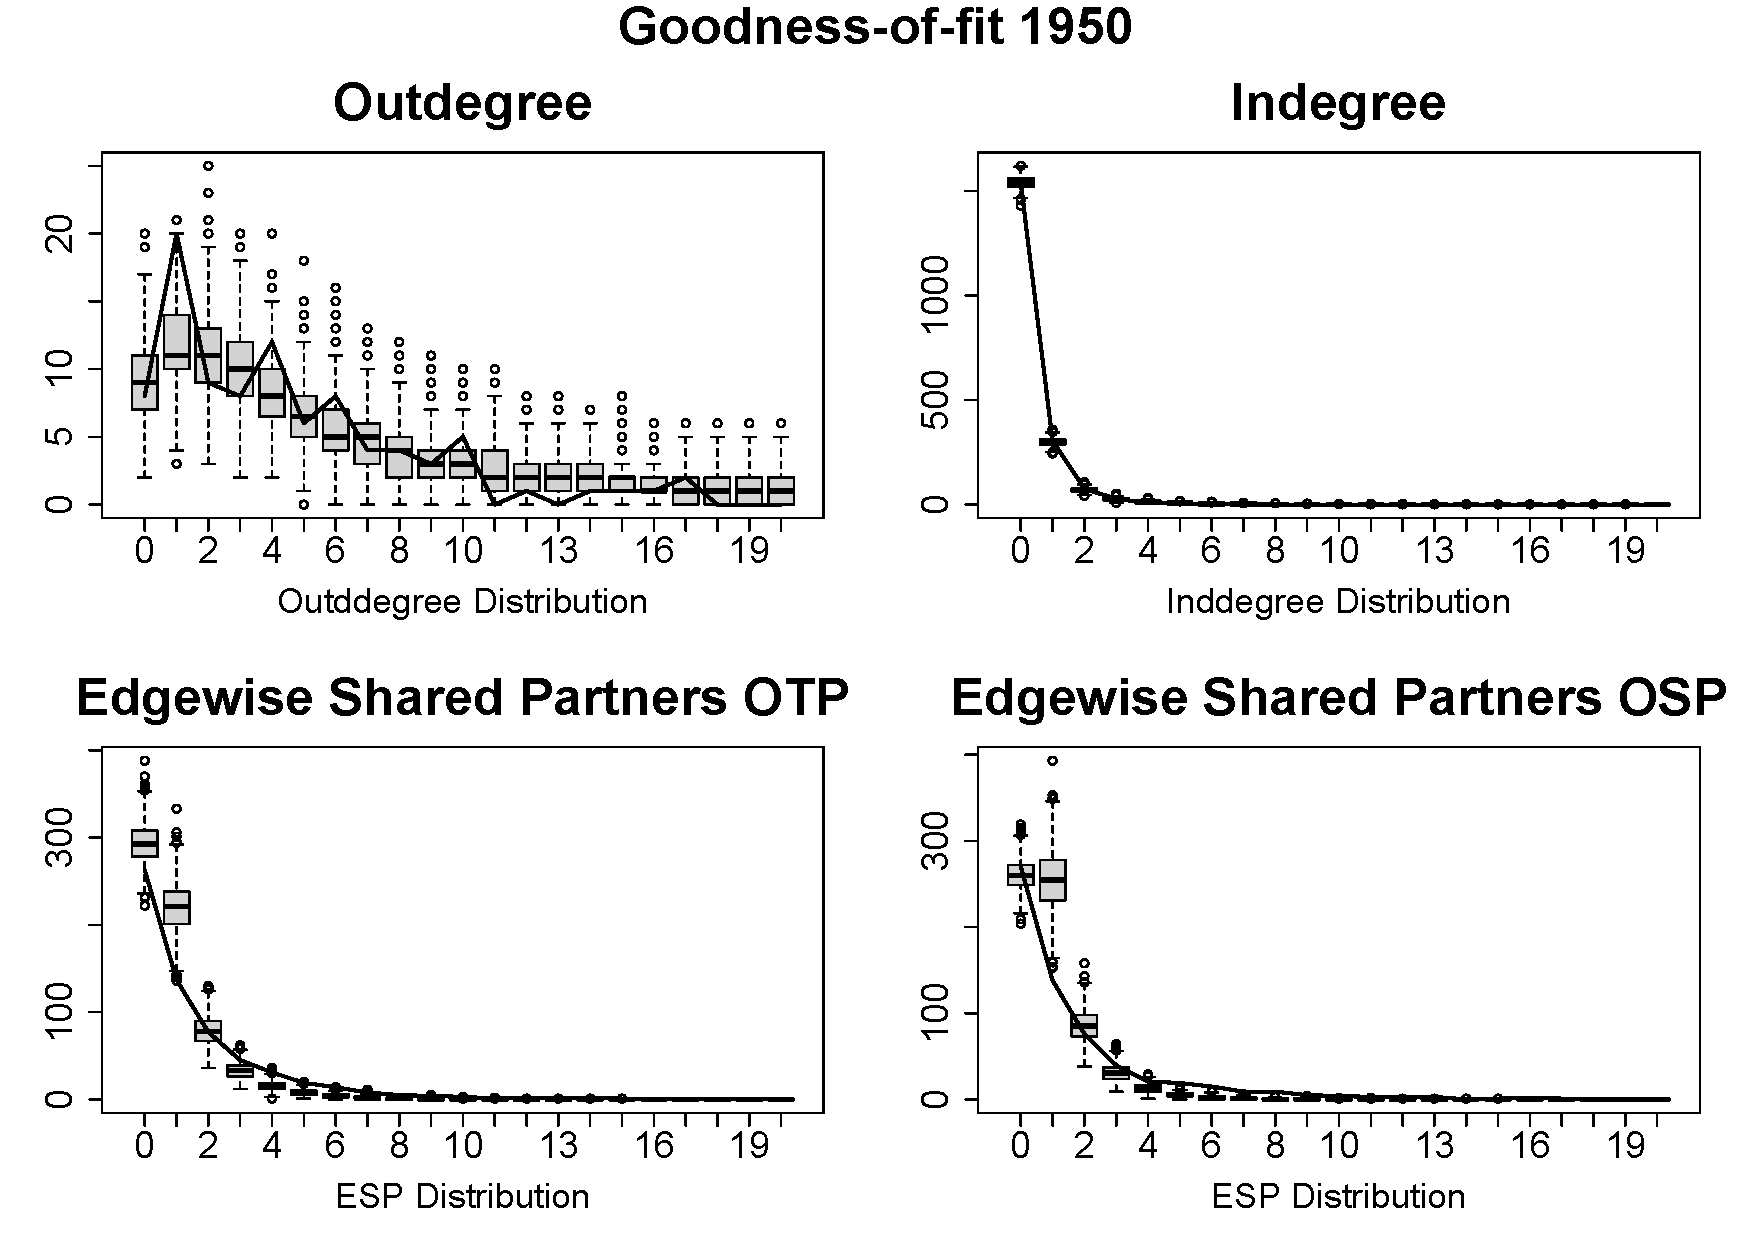
\includegraphics[width=13.8cm]{GOF_1950}\\
%\caption{Goodness-of-fit diagnostic for the 1950 network.}
% \label{GOF_1950}
\vspace{1cm}
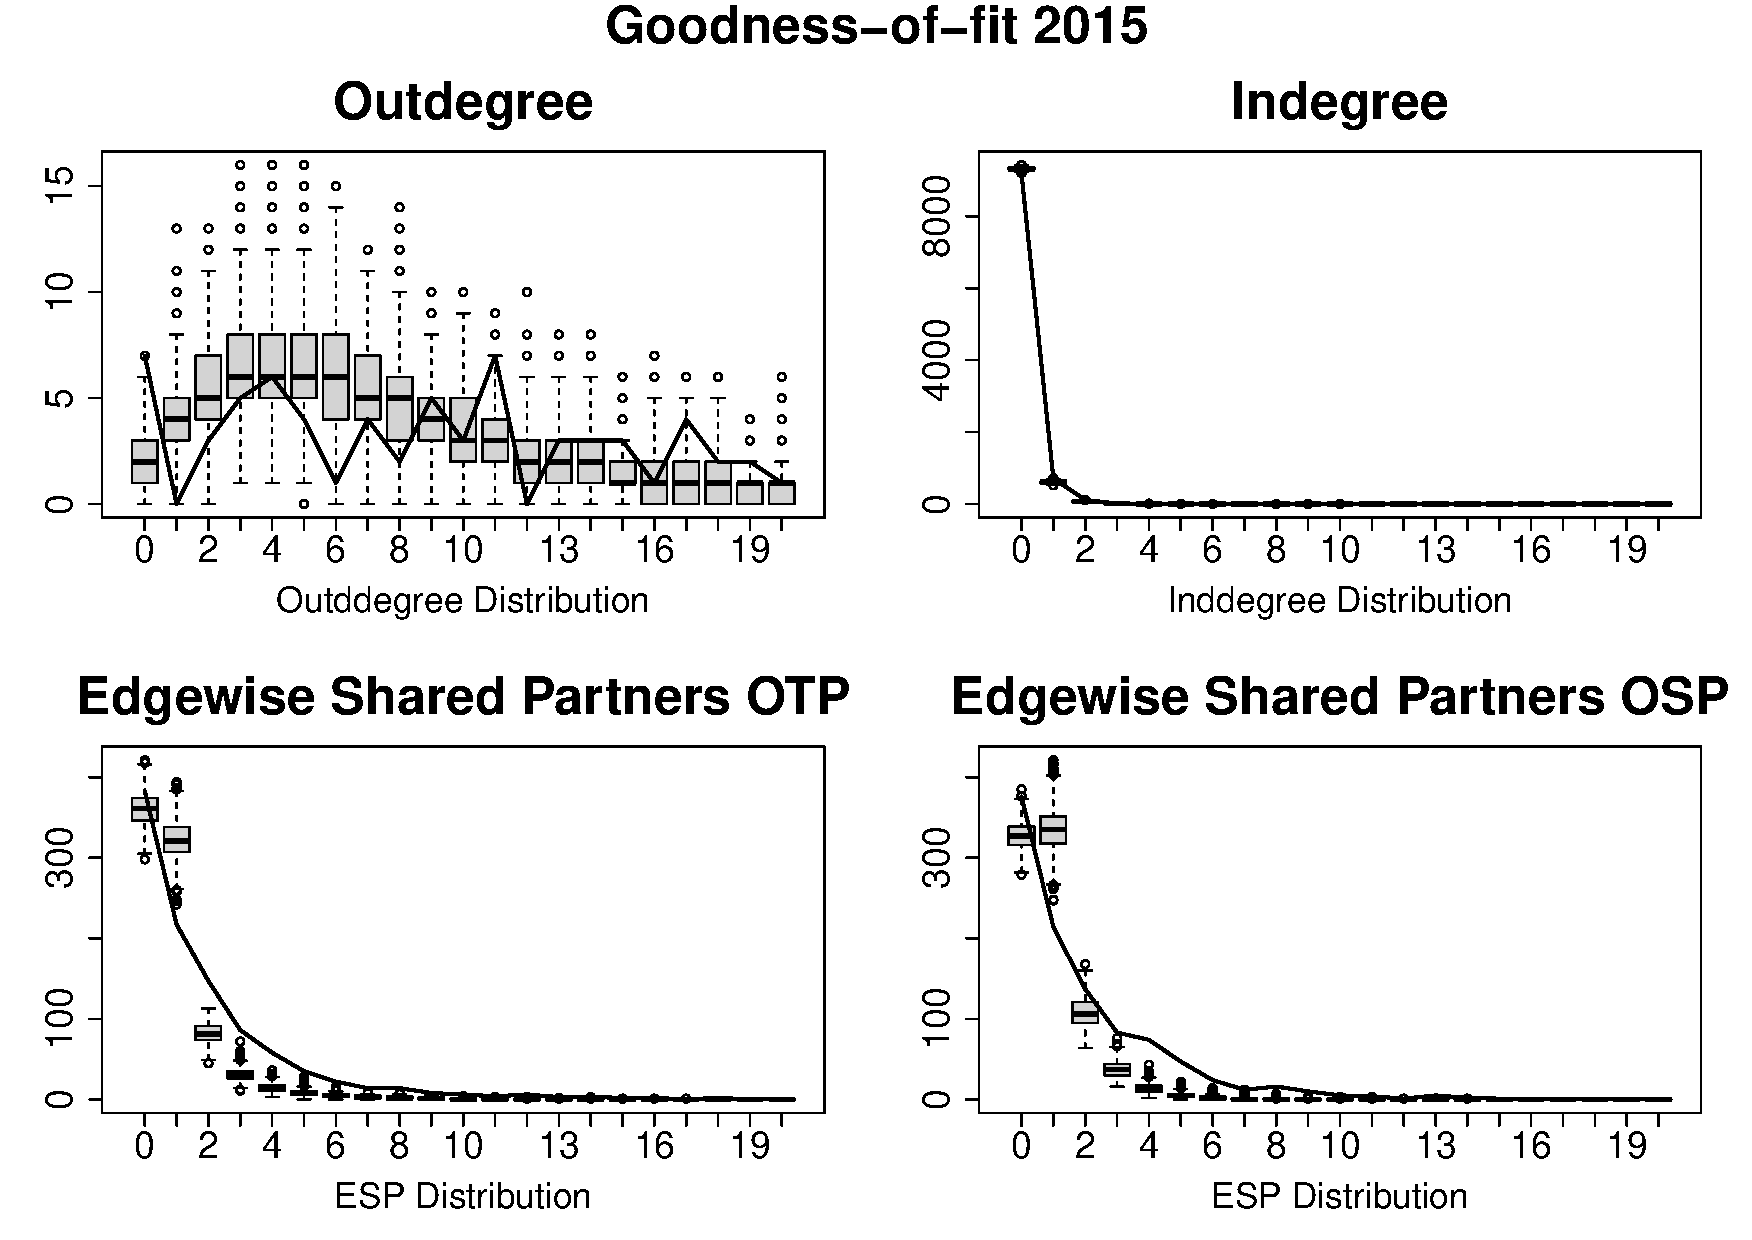
\includegraphics[width=13.8cm]{GOF_2015}
\vspace{0.1cm}
\caption{Goodness-of-fit diagnostic for the 1950 network (top) and the 2015 network (bottom).}
 \label{GOF}
\vspace{-.25cm}
\end{center}
\end{figure} 


\section{Checking for Model Degeneracy}

A common challenge when fitting ERGMs is model degeneracy. Model degeneracy occurs when the probability distribution defined by the parameter vector does not predominantly yield networks with similar statistics as the observed network. Generally, model degeneracy results in simulated networks with no ties or all possible ties. In a non-degenerate model the statistics of the networks that were simulated from the probability distribution defined by the MCMLE fall in the proximity of the observed network's statistics. Figures \ref{mcmcdiagnostics_1950} and \ref{mcmcdiagnostics_2015} depict trace and density plots for the dependence terms in the 1950 and 2015 term citation network. The histograms on the left visualize a statistic's density from $1000$ simulated networks, while the right side shows the statistic's trace plot of the same $1000$ networks. The solid black line indicates the statistic's value in the actual citation network. Both figures indicate that this model is non-degenerate and that the simulated network's statistics fall almost evenly around the observed statistic. The density and trace plots for the ERGM of the terms not depicted provide similar results.

\bibliography{bib} 
\bibliographystyle{apsr}

\begin{figure}[H]
 \begin{center}
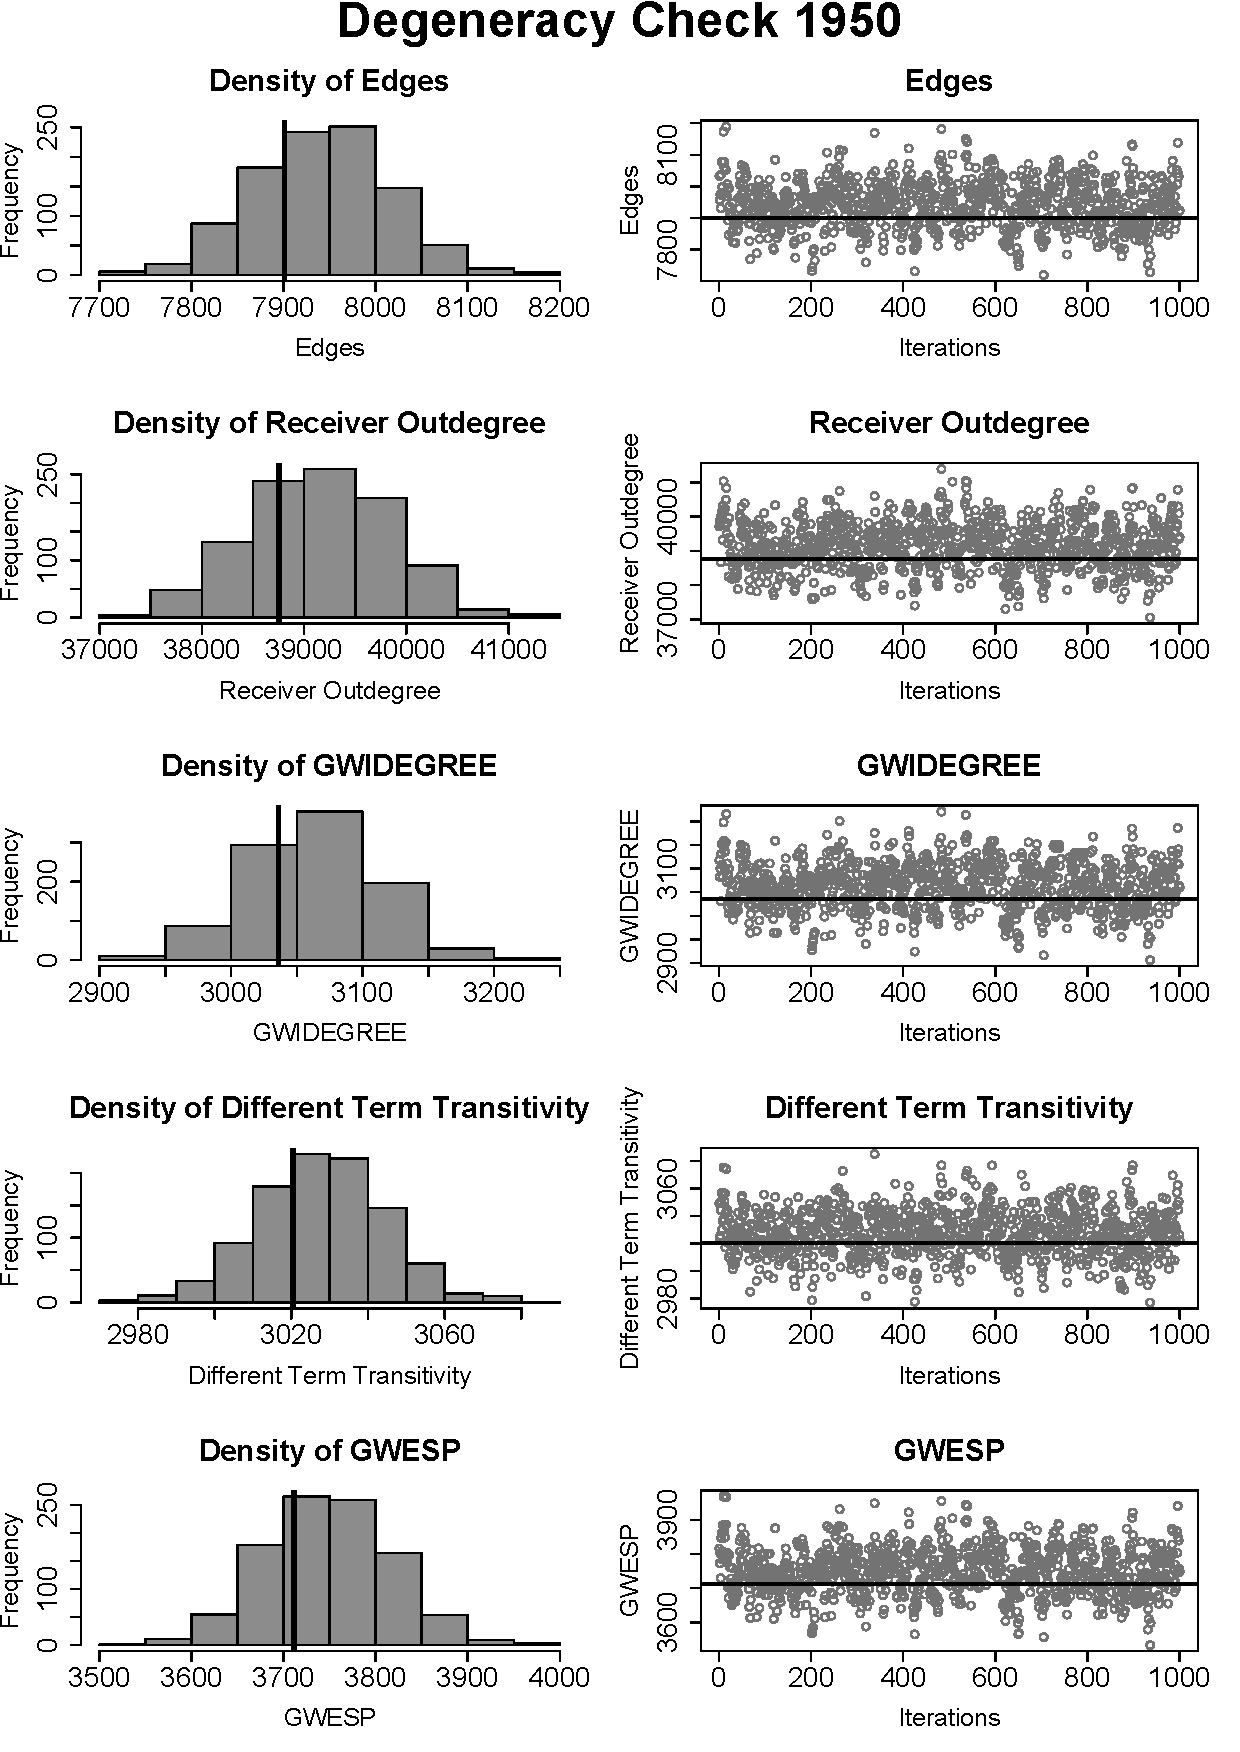
\includegraphics[width=14.5cm]{Deg_1950}
\caption{Density and trace plots for the dependency terms of the 1950 term citation network.}
 \label{mcmcdiagnostics_1950}
\vspace{-.25cm}
\end{center}
\end{figure} 


 \begin{figure}[H]
 \begin{center}
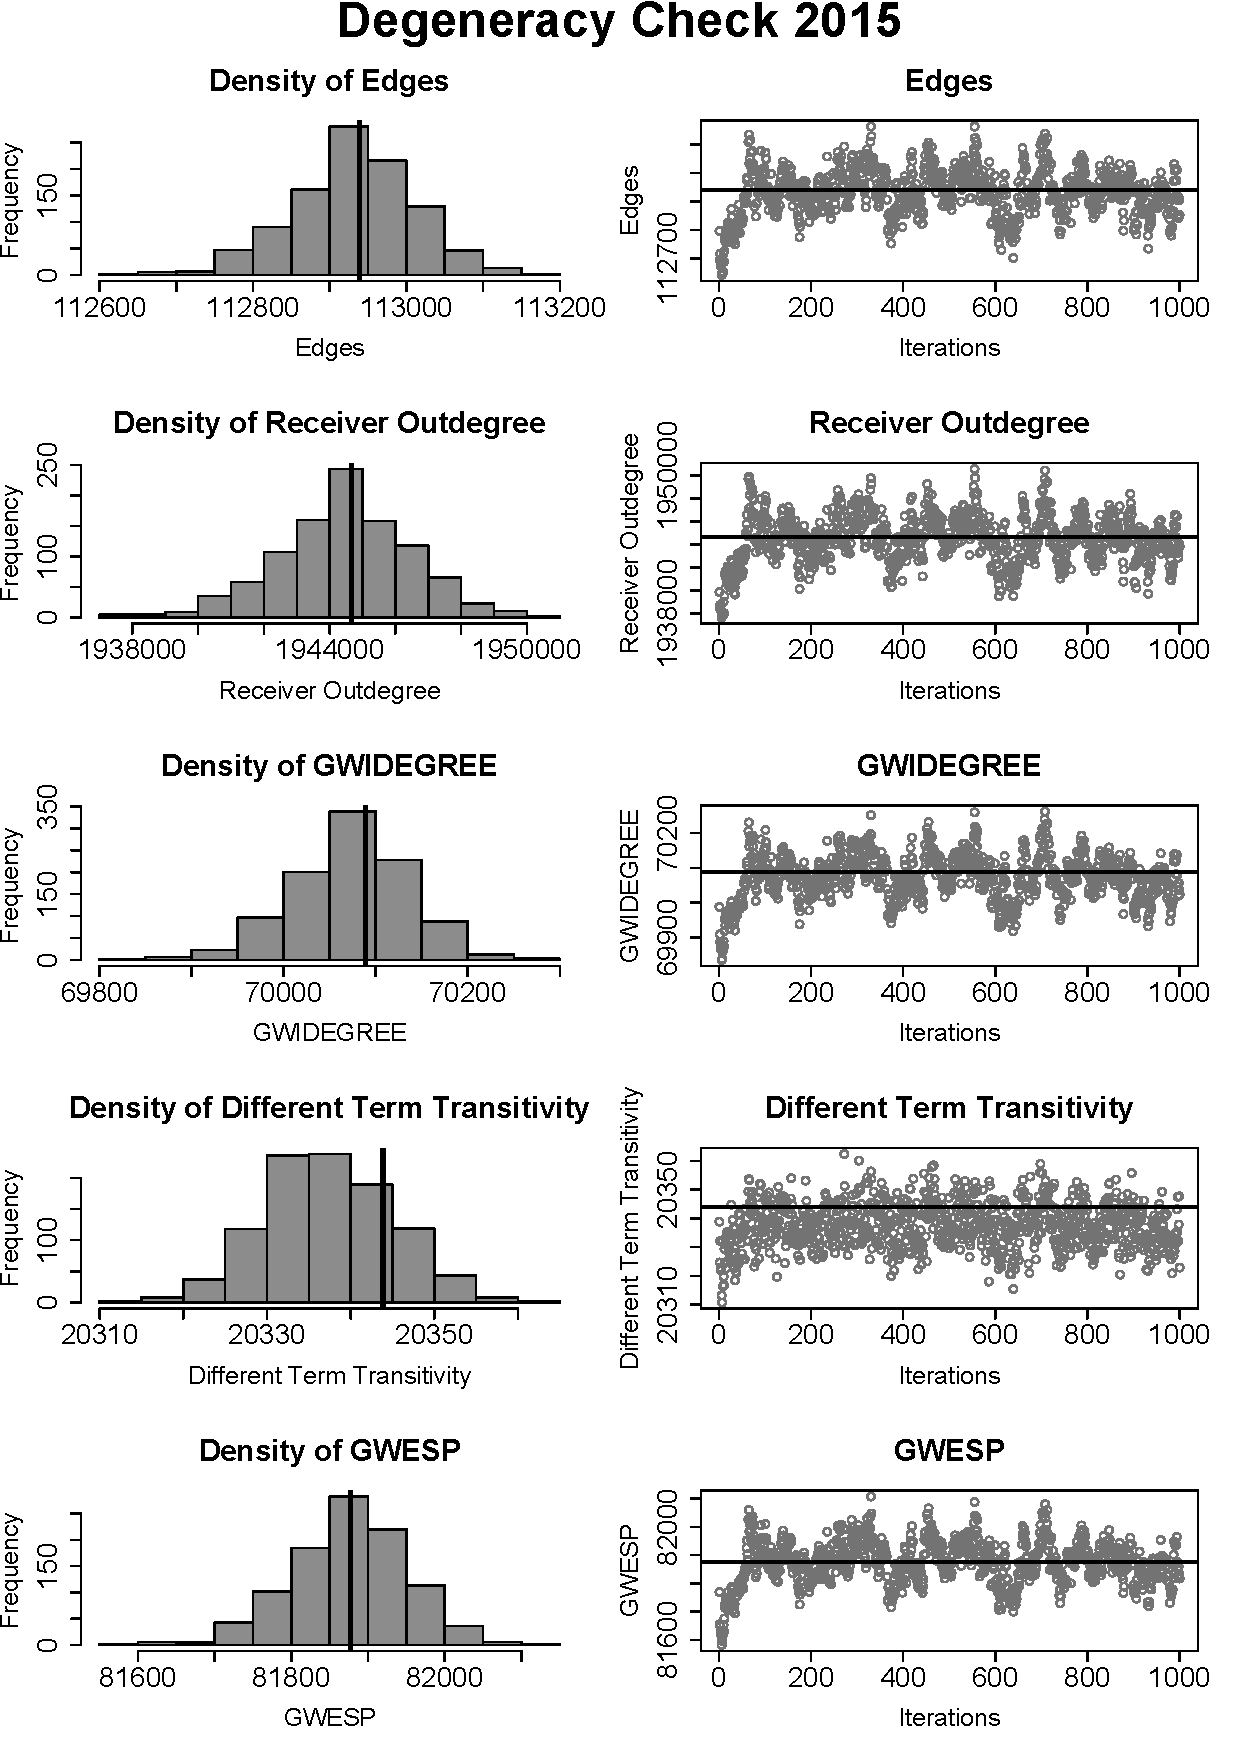
\includegraphics[width=14.5cm]{Deg_2015}
\caption{Density and trace plots for the dependency terms of the 2015 term citation network.}
 \label{mcmcdiagnostics_2015}
\vspace{-.25cm}
\end{center}
\end{figure} 





\end{document}




















